\chapter{The Physical Layer}
\label{cha:physicallayer}

\section{Overview}

Today's electric devices use more and more wireless communication methods such
as Wifi, Bluetooth, NFC, UMTS, and LTE. Despite the diversity of these devices
there are many similarities in the modeling of their physical layer components.
The models often have similar signal representations and signal processing steps,
and they also share the physical medium model where communication takes place.

In general, the physical layer simulation is a very time consuming task. The
simulation of signal propagation, signal fading, signal interference, and signal
decoding in detail may often result in unacceptable performance. Finding the
right abstractions, the right level of detail, and the right trade-offs between
accuracy and performance is difficult and very important.

To summarize, the physical layer is designed with the following goals in mind:
\begin{itemize}
  \item customizability
  \item extensibility
  \item scalable level of detail
  \item ability to exploit parallel hardware
\end{itemize}

The following sections provide a brief overview of the physical layer model. For
more details on the available modules, their parameterization and the actual
implementations please refer to the documentation in the corresponding NED and
C++ source files.

\subsection{Customizability}

Real world communication devices often provide a wide variety of configuration
options to allow adapting to the physical conditions where they are required
to operate. For example, a Wifi router administration interface often provides
parameters to configure the transmission power, bitrate, preamble type, carrier
frequency, RTS threshold, beacon interval, etc. Mostly these parameters have
default values assigned, so the user doesn't have to set them separately, but
may override them as needed.

Similarly to real world devices the physical layer models also provide a wide
variety of parameters to control their behavior. The most common NED parameters
are various physical quantities with physical units such as transmission power
\ttt{[W]}, reception sensitivity \ttt{[W]}, carrier frequency \ttt{[Hz]},
communication range \ttt{[m]}, propagation speed \ttt{[m/s]}, SNIR reception
threshold \ttt{[dB]}, bitrate \ttt{[b/s]}. Occasionally models support new
parameters or new combinations, which don't exist in real world hardware, to
allow further experimentation.

Another important and commonly used parameter kind selects among alternative
implementations of a particular interface by providing its name. Different
implementations are often separate modules, which come with their own set of
parameters to avoid the confusion of mixing their unrelated parameters. Some
modules may be split into more submodules. This further deepens the module
hierarchy, but allows better extensibility.

\subsection{Extensibility}

Similarly to designing other simulation models, modeling the physical layer is
not at all an unambiguous task. For example, the research literature contains a
number of different path loss models for signal propagation, there are different
bit error models for a particular protocol standard, representing the signal in
the analog domain can also be done in several different ways, and so on.

In order to support this diversity the physical layer is designed to be
extensible with alternative implementations at various parts of the model. This
is realized by separately defining C++ and NED interfaces between modules, and
also by providing parameters in their parent modules to easily select among the
available implementations.

New models can be added by implementing the required interfaces from scratch, or
by deriving from already existing implementations and overriding functionality.
This architecture allows the user to create new models with less effort, and to
focus on the real differences, while the rest of the physical layer remains the
same.

\subsection{Scalable Level of Detail}

There are many possible ways to model various aspects of the physical layer.
The most important difference lies in the trade-off between performance versus
accuracy. In order to support the different trade-offs the physical layer is
designed to be scalable with respect to the simulated level of detail. In other
words, it's scalable from high-performance less accurate simulations to high
fidelity slower simulations.

The physical layer model is scalable along the following axes:

\begin{itemize}
  \item simulation model
  \item software architecture
  \item data representation
  \item number of messages
\end{itemize}

The simulation model might vary from simple statistical models to accurate
emulation. The simplest models ignore the actual bits of the transmission. For
example, the extremely simple unit disc radio even ignores the signal power. The
most accurate models use precise signal representation for all four domains:
bit domain, symbol domain, sample domain, and analog domain representations.
They also emulate most functions of real hardware in detail: forward error
correction, interleaving, scrambling, modulation, spreading, pulse shaping, and
so on.

The software architecture might vary from flat to layered. A flat architecture
is efficient but not modular. Functionality can only be affected through simple
parameters and not by providing alternative implementations. Whereas a layered
architecture is more flexible at the cost of more complex data structures, more
data conversions, more resource management, and thus slower processing. On the
other hand, it provides more customization opportunities to replace parts with
alternative implementations and to do research easier in the area.

The data representation might vary from scalar to multidimensional values. In
the analog domain of the physical layer data quite often changes over time,
frequency, space, or any combination thereof. The most obvious example is the
analog signal power, but there are others such as signal phase or the signal to
noise ratio.

The number of messages per transmission added to the future event queue might
vary from one to the number of radios. One message might be sufficient, for
example, if the transmission is intended to a single destination, and other
receivers are either not affected, or the effect is negligible. On the other
hand, it might be necessary to process all transmissions by all receivers in
order to have the desired effect on the higher layers. For example, if a MAC
model is configured to promiscuous mode, it needs to receive all transmissions.

\subsection{Exploiting Parallel Hardware}

The physical processes simulated by the physical layer are inherently parallel.
The computation of the transmission arrival space-time coordinates, the analog
signal representation of transmissions and receptions, the interfering
receptions and noises, the signal to noise ratio, the decoded bits, the bit
errors, and the physical layer indications all provide a good parallelization
opportunity, because they dominate the physical layer performance and are
independent for each receiver. Therefore the physical layer is designed to be
able to utilize parallel hardware, multi-core CPUs, vector instructions and the
highly parallel GPU.

The idea is to have a central component in the software architecture where
parallel computation can happen. This central component is the medium model
that knows about all radios, transmissions, interferences, and receptions
anyway. It uses optimistic parallel computation in multiple background threads
while the main simulation thread continues normal execution. When a new
transmission enters the channel the already computed and affected results are
invalidated or updated, and the affected ongoing optimistic parallel
computations are canceled.

\section{The Radio Model}

The radio model describes the physical device that is capable of transmitting
and receiving signals on the medium. It contains an antenna model, a transmitter
model, a receiver model, and an energy consumer model. The antenna model is
shared between the transmitter model and the receiver model. The separation of
the transmitter model and the receiver model allows asymmetric configurations.
The energy consumer model is optional and it's only used when the simulation of
energy consumption is necessary.

The radio model has an operational mode that is called the radio mode. The radio
mode is externally controlled usually by the MAC model. In transceiver mode, the
radio can simultaneously transmit and receive a signal. Changing the radio mode
may optionally take a non-zero amount of time. The supported radio modes are the
following:

\begin{itemize}
  \item \ttt{off}: communication isn't possible, energy consumption is zero
  \item \ttt{sleep}: communication isn't possible, energy consumption is minimal
  \item \ttt{receiver}: only reception is possible, energy consumption is low
  \item \ttt{transmitter}: only transmission is possible, energy consumption is
high
  \item \ttt{transceiver}: reception and transmission is simultaneously
possible, energy consumption is high
  \item \ttt{switching}: communication isn't possible, energy consumption is
minimal
\end{itemize}

In addition to the radio mode, the transmitter and the receiver models have
separate states which describe what they are doing. Changes to these states are
automatically published by the radio. The signaled transmitter states are the
following:

\begin{itemize}
  \item \ttt{undefined}: isn't operating
  \item \ttt{idle}: there's no transmission in progress
  \item \ttt{transmitting}: transmission is in progress
\end{itemize}

The signaled receiver states are the following:

\begin{itemize}
  \item \ttt{undefined}: isn't operating
  \item \ttt{idle}: there's no reception in progress
  \item \ttt{busy}: received signal is not interpretable
  \item \ttt{synchronizing}: synchronization is in progress
  \item \ttt{receiving}: reception is in progress
\end{itemize}

When a radio wants to transmit a signal on the medium it sends direct messages
to all affected radios with the help of the central medium module. The messages
contain a shared data structure which describes the transmission the way it
entered the medium. The messages arrive at the moment when start of the
transmission arrive at the receiver. The receiver radios also handle the
incoming messages with the help of the central medium module. This kind of
centralization allows the medium to do shared computations in a more efficient
way and it also makes parallel computation possible.

As stated above the radio module utilizes multiple submodules to further split
its task. This design decision makes it more extensible and customizable. The
following sections describe the parts of the radio model.

\subsection{Antenna Models}

The antenna model describes the effects of the physical device which converts
electric signals into radio waves, and vice versa. This model captures the
antenna characteristics that heavily affect the quality of the communication
channel. For example, various antenna shapes, antenna size and geometry, antenna
arrays, and antenna orientation causes different directional or frequency
selectivity.

The antenna model provides a position and an orientation using a mobility model
that defaults to the mobility of the node. The main purpose of this model is to
compute the antenna gain based on the specific antenna characteristics and the
direction of the signal. The signal direction is computed by the medium from the
position and the orientation of the transmitter and the receiver. The following
list provides some examples:

\begin{itemize}
  \item \nedtype{IsotropicAntenna}: antenna gain is exactly 1 in any direction
  \item \nedtype{ConstantGainAntenna}: antenna gain is a constant determined by
a parameter
  \item \nedtype{DipoleAntenna}: antenna gain depends on the direction according
to the dipole antenna characteristics
  \item \nedtype{InterpolatingAntenna}: antenna gain is computed by linear
interpolation according to a table indexed by the direction angles
\end{itemize}

The antenna models are in the \ttt{src/physicallayer/antenna/} directory.

\subsection{Transmitter Models}

The transmitter model describes the physical process which converts packets into
electric signals. In other words, this model converts a MAC packet into a signal
that is transmitted on the medium. The conversion process and the representation
of the signal depends on the level of detail and the physical characteristics
of the implemented protocol.

In the flat model the transmitter model skips the symbol domain and the sample
domain representations, and it directly creates the analog domain representation.
The bit domain representation is reduced to the bit length of the packet and the
actual bits are ignored.

In the layered model the conversion process involves various processing steps
such as packet serialization, forward error correction encoding, scrambling,
interleaving, and modulation. This transmitter model requires much more
computation, but it produces accurate bit domain, symbol domain, and sample
domain representations.

The various protocol specific transmitter models are in the corresponding
directories.

\subsection{Receiver Models}

The receiver model describes the physical process which converts electric
signals into packets. In other words, this model converts a reception, along
with an interference computed by the medium model, into a MAC packet and a
reception indication. It also determines the following for each transmission: 

\begin{itemize}
  \item \ttt{is the reception possible or not}: based on the signal
characteristics such as reception power, carrier frequency, bandwidth, preamble
mode, modulation scheme
  \item \ttt{if the reception is possible, is reception attempted or not}: based
on the ongoing reception and the support of signal capturing
  \item \ttt{if the reception is attempted, is reception successful or not}:
based on the error model and the simulated part of the signal decoding
\end{itemize}

In the flat model the receiver model skips the sample domain, the symbol domain,
and the bit domain representations, and it directly creates the packet domain
representation by copying the packet from the transmission. It uses the error
model to decide if the reception is successful or not.

In the layered model the conversion process involves various processing steps
such as demodulation, descrambling, deinterleaving, forward error correction
decoding, and deserialization. This reception model requires much more
computation, but it produces accurate sample domain, symbol domain, and bit
domain representations.

The various protocol specific receiver models are in the corresponding 
directories.

\subsection{Error Models}

Determining the reception errors is a crucial part of the reception process.
There are often several different statistical error models in the literature
even for a particular physical layer. In order to support this diversity the
error model is a separate replaceable component of the receiver. 

The error model describes how the signal to noise ratio affects the amount of
errors at the receiver. The main purpose of this model is to determine whether
if the received packet has errors or not. It also computes various physical
layer indications for higher layers such as packet error rate, bit error rate,
and symbol error rate. For the layered reception model it needs to compute the
erroneous bits, symbols, or samples depending on the lowest simulated physical
domain where the real decoding starts. The error model is optional, if omitted
all receptions are considered successful.

The error models are in the \ttt{src/physicallayer/errormodel/} directory and
also in the corresponding protocol specific directories.

\subsection{Energy Consumer Models}

A substantial part of the energy consumption of communication devices comes from
transmitting and receiving signals. The energy consumer model describes how the
radio consumes energy depending on its activity. This model is optional, if
omitted energy consumption is ignored. The following list provides some examples:

\begin{itemize}
  \item \nedtype{StateBasedEnergyConsumer}: the constant power consumption is
determined by valid combinations of the radio mode, the transmitter state and
the receiver state
\end{itemize}

The energy consumer models are in the \ttt{src/physicallayer/energyconsumer/} directory.

\ifdraft
TODO: layered
\subsection{Layered Radio Model}

This module further splits the transmitter and receiver models to allow bit
precise communication modeling.

TODO: layered

The following sections describe the parts of the layered radio model.

\subsubsection{Encoding and Decoding}

This module describes how the packet domain signal representation is converted
into the bit domain, and vice versa.

TODO: layered

\subsubsection{Modulation and Demodulation}

This module describes how the bit domain signal representation is converted into
the symbol domain, and vice versa.

TODO: layered

\subsubsection{Pulse Shaping and Pulse Filtering}

This module describes how the symbol domain signal representation is converted
into the sample domain, and vice versa.

TODO: layered


\subsubsection{Digital Analog and Analog Digital Conversion}

This module describes how the sample domain signal representation is converted
into the analog domain, and vice versa.

TODO: layered
\fi

\section{The Medium Model}

The medium model describes the shared physical medium where communication takes
place. It keeps track of radios, noise sources, ongoing transmissions,
background noise, and other ongoing noises. The medium computes when, where and
how transmissions and noises arrive at receivers. It also efficiently provides
the set of interfering transmissions and noises for the receivers. It doesn't
send or handle messages on its own, it rather acts as a mediator between radios.

The medium model provides a couple of parameters to optimize for performance.
For example, the filter parameters control how the model determines the set of
affected radios when a new transmission enters the medium. The medium model
maintains the following global limits among the registered radios to support
various optimizations:

\begin{itemize}
  \item maximum speed
  \item maximum antenna gain
  \item maximum transmission power
  \item minimum interference power
  \item minimum reception power
  \item minimum interference time
  \item maximum transmission duration
  \item maximum detection range
  \item maximum interference range
  \item maximum communication range
  \item minimum and maximum mobility constraints
\end{itemize}

The medium module utilizes multiple submodules to further split its task. This
design makes it extensible and customizable. The following sections describe
the parts of the medium.

\subsection{Propagation Models}

Whenever the radio transmits a signal, it starts to propagate through space. The
transmitter might move during the transmission interval, and the receiver might
also move during both the propagation time and the reception interval. The
effect of these movements becomes more and more important as the propagation
speed and the speed of the radios gets closer to each other. This is especially
true for acoustic communication because the propagation speed of the signal is
much smaller. In general, it's difficult to accurately compute the signal
arrival, but it's usually not really necessary, some kind of approximation
suffices.

The propagation model is a separate component of the medium model to make it
extensible with alternative implementations. This model describes how signals
propagate through space over time. The main purpose of this model is to compute
the arrival space-time coordinates for transmissions. The following list
provides some examples:

\begin{itemize}
  \item \nedtype{ConstantTimePropagation}: propagation time is independent of
the traveled distance and it's determined by a constant parameter
  \item \nedtype{ConstantSpeedPropagation}: propagation time is proportional to
the traveled distance determined by a constant propagation speed parameter
\ifdraft
TODO: parallel
  \item \nedtype{ConstantSpeedGPUPropagation}: propagation time is computed in
parallel on the GPU for all receivers
\fi
\end{itemize}

The propagation models are in the \ttt{src/physicallayer/propagation/} directory.

\subsection{Path Loss Models}

As the signal propagates through space its power density decreases. Path loss
might be due to the combination of many effects, such as free-space loss,
refraction, diffraction, reflection, and absorption. There are several different
models in the literature, which differ in their parameterization and application
area.

The path loss model is a separate component of the medium model to make it
extensible with alternative implementations. This model describes the reduction
of power as the signal propagates through space. It computes the power loss
factor based on the traveled distance, the signal frequency and the propagation
speed. It may also provide the opposite, that is the traveled distance based on
the power loss factor, the signal frequency and the propagation speed. The
latter computation is useful for determining the maximum communication range
based on the transmission power and the reception sensitvity. The following list
provides some examples:

\begin{itemize}
  \item \nedtype{FreeSpacePathLoss}
  \item \nedtype{LogNormalShadowing}
  \item \nedtype{TwoRayGroundReflection}
  \item \nedtype{BreakpointPathLoss}
  \item \nedtype{NakagamiFading}
  \item \nedtype{RayleighFading}
  \item \nedtype{RicianFading}
  \item \nedtype{SUIPathLoss}
  \item \nedtype{UWBIRStochasticPathLoss}
  \item etc.
\end{itemize}

The path loss models are in the \ttt{src/physicallayer/pathloss/} directory.

\subsection{Obstacle Loss Models}

When the signal propagates through space it also passes through physical objects
present in that space. As the signal passes through, its power decreases when it
reflects from the surfaces of physical objects, and also when it's absorbed by
their material. There are various ways to model this effect, which differ in the
trade-off between accuracy and performance.

The obstacle loss model is a separate component of the medium model to make it
extensible with alternative implementations. This model describes the reduction
of power as the signal passes through physical objects. The main purpose of this
model is to compute the power loss factor based on the traveled straight path,
the signal frequency and the physical properties of the obstructing physical
objects. The obstacle model utilizes the physical environment model to query the
obstructing physical objects. The following list provides some examples:

\begin{itemize}
  \item \nedtype{TracingObstacleLoss}: the power loss is based on computing the
accurate dielectric and reflection loss along the straight path considering the
shape, the position, the orientation, and the material of obstructing physical
objects
\end{itemize}

The obstacle loss models are in the \ttt{src/physicallayer/obstacleloss/}
directory.

\ifdraft
TODO: multipath
\subsection{Multipath Models}

The signal reflects from the surfaces, it refracts as it passes through the
surfaces, it diffracts as it passes around the objects. 

The multipath model describes the alternative paths that the signal travels
before it either reaches the receiver or sufficiently fades.
\fi

\subsection{Background Noise Models}

The thermal noise, the cosmic background noise, and other random fluctuations of
the electromagnetic field affect the quality of the communication channel. This
kind of noise doesn't come from a particular source and it doesn't propagate
through space.

The background noise model is a separate component of the medium model to make
it extensible with alternative implementations. This model describes how the
background noise changes over space and time. The main purpose of this model is
to compute the analog representation of the noise signal for a given space-time
interval.

\begin{itemize}
  \item \nedtype{IsotropicBackgroundNoise}: the background noise is independent
of the time and the position, and its power is determined by a constant parameter 
\end{itemize}

The background noise models are in the \ttt{src/physicallayer/backgroundnoise/}
directory.

\subsection{Neighbor Cache Models}

Transceivers are considered neighbors if successful communication is possible
between them. In wired communication systems it's mostly quite obvious which
transceivers are neighbors, because they are connected by wires. In contrast,
in wireless communication systems determining which radios are neighbors isn't
obvious at all. 

The neighbor cache model is a separate component of the medium model to make it
extensible with alternative implementations. This model provides an efficient
way of keeping track of the neighbor relationship between radios. The main
purpose of this model is to compute the affected set of receivers on the medium
for a given transmission. The model also has to follow the movement of radios,
but it might provide conservative approximations for queries. The following list
provides some examples:

\begin{itemize}
  \item \nedtype{NeighborListNeighborCache}: maintains a separate periodically
updated  neighbor list for each radio
  \item \nedtype{GridNeighborCache}: organizes radios in a 3 dimensional grid
with constant cell size and updates periodically
  \item \nedtype{QuadTreeNeighborCache}: organizes radios in a 2 dimensional
quad tree (ignoring the Z axis) with constant node size and updates periodically
\end{itemize}

The neighbor cache models are in the \ttt{src/physicallayer/neighborcache/}
directory.

\section{Signal Representation}

The data structures that represent the transmitted and the received signals
might contain many different data depending on the simulated level of detail. In
addition, the reception data structure might contain various physical layer
indications, which are computed during the reception process. The following list
provides some examples:

\begin{itemize}
  \item \ttt{packet domain}: actual packet, packet error rate, packet error bit,
etc.
  \item \ttt{bit domain}: various bit lengths, bitrates, actual bits, forward
error correction code, interleaving scheme, scrambling scheme, bit error rate,
number of bit errors, actual erroneous bits, etc.
  \item \ttt{symbol domain}: number of symbols, symbol rate, actual symbols,
modulation scheme, symbol error rate, number of symbol errors, actual erroneous
symbols, etc.
  \item \ttt{sample domain}: number of samples, sampling rate, actual samples,
etc.
  \item \ttt{analog domain}: space-time coordinates, antenna orientations,
communication range, interference range, detection range, carrier frequency,
subcarrier frequencies, bandwidths, scalar or dimensional power, receive signal
strength indication, signal to noise and interference ratio, etc.
\end{itemize}

In simple case the packet domain specifies the MAC packet only, and the bit
domain specifies the bit length and the bitrate. The symbol domain specifies the
used modulation, and the sample domain is simply ignored. The most important
part is the analog domain representation, because it's indispensable to be able
to compute some kind of signal to noise and interference ratio. The following
figure shows four different kinds of analog domain representations, but other
representations are also possible.

\begin{figure}[h!]
\centering
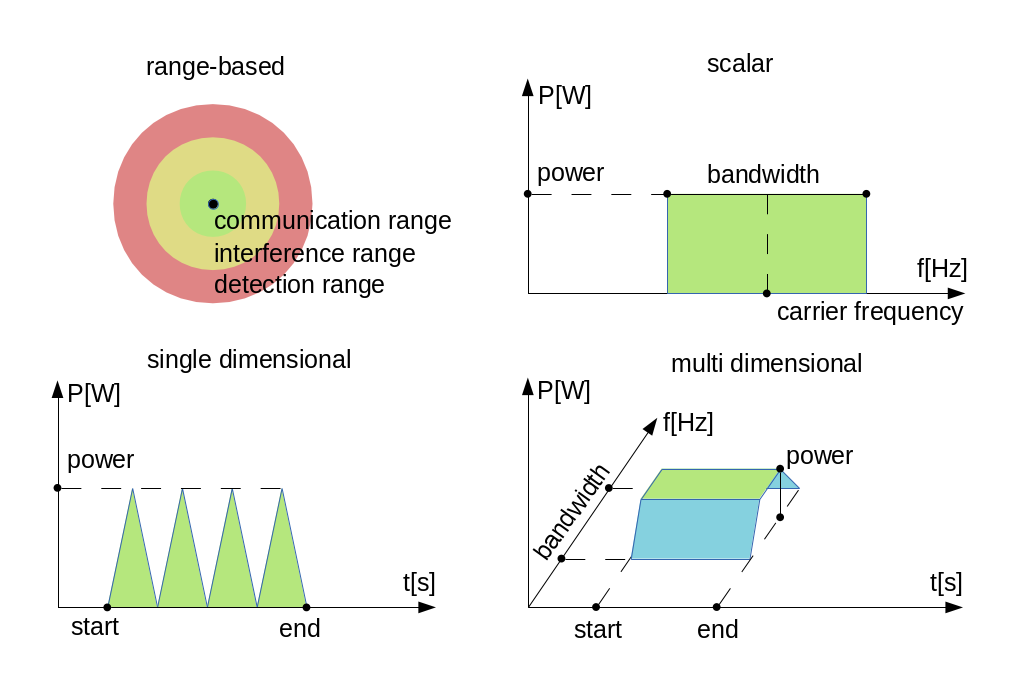
\includegraphics[width=\textwidth]{figures/phyanalog}
\caption{Various analog signal representations}
\end{figure}

The first representation is called range-based, and it's used by the unit disc
radio. The advantage of this data structure is that it's compact, predictable,
and provides high performance. The disadvantage is that it's very inaccurate in
terms of modeling reality. Nevertheless, this representation might be sufficient
for developing a new routing protocol if accurate simulation of packet loss is
not important.

The second data structure represents a narrowband signal with a scalar signal
power, a carrier frequency, and a bandwidth. The advantage of this
representation is that it allows to compute a real signal to noise ratio, which
in turn can be used by the error model to compute bit and packet error rates.
This representation is most of the time sufficient for the simulation of IEEE
802.11 networks.

The third data structure describes a signal power that changes over time. In
this case the signal power is represented with a one-dimensional time dependent
value that precisely follows the transmitted pulses. This representation is used
by the IEEE 802.15.4a UWB radio.

The last representation uses a multi-dimensional value to describe the signal
power that changes over both time and frequency. The IEEE 802.11b model might
use this representation to simulate crosstalk, where one channel interferes with
another. In order to make it work the frequency spectrum of the signal has to
follow the real spectrum more precisely at both ends of the band.

The flat signal representation uses a single object to simulatenously describe
all domains of the transmission or the reception. In contrast, the layered
signal representation uses one object to describe every domain seperately. The
advantage of the latter is that it's extensible with alternative implementations
for each domain. The disadvantage is that it needs more allocation and resource
management.

\section{Signal Processing}

The following figure shows the process of how a MAC packet gets from the
transmitter radio through the medium to the receiver radio. The figure focues on
how data flows between the processing components of the physical layer. The blue
boxes represent the data structures, and the red boxes represent the processing
components.

\begin{figure}[h!]
\centering
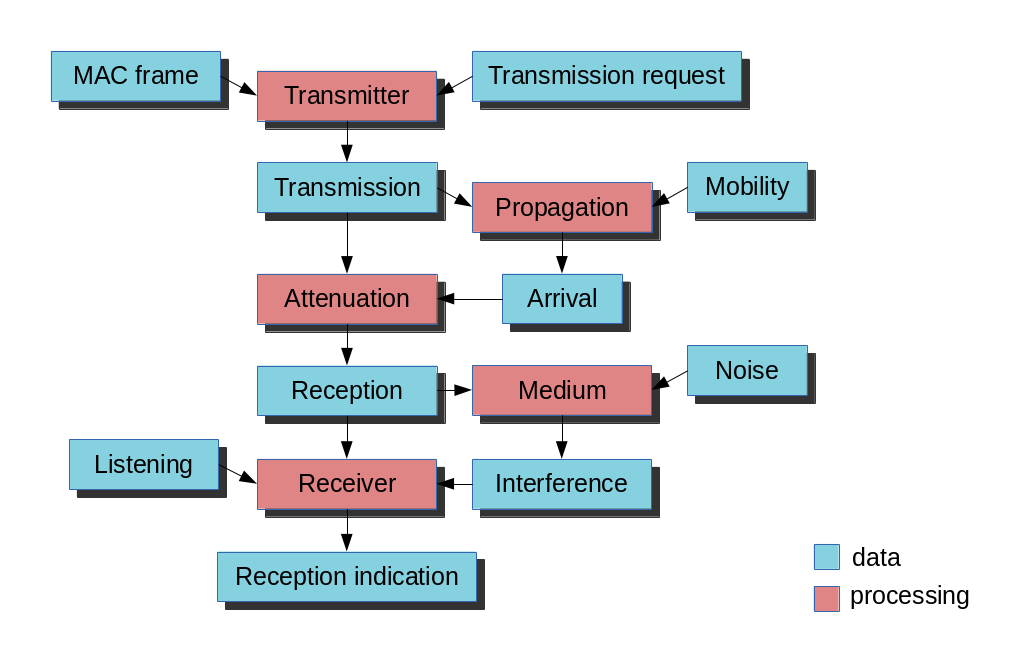
\includegraphics[width=\textwidth]{figures/phydataflow}
\caption{Signal processing data flow}
\end{figure}

The transmission process starts in the transmitter radio when it receives a MAC
packet from the higher layer. The radio must be in transmitter or transceiver
mode before receiving a MAC packet, otherwise it throws an exception. At first
the transmitter model creates a data structure that describes the transmitted
signal based on the received MAC packet and the attached transmission request.
The resulting data structure is immutable, it's not going to be changed in any
later processing step.

Thereafter the propagation model computes the arrival space-time coordinates for
all receivers. In the next step the medium model determines the set of affected
receivers. Which radio constitutes affected depends on a number of factors such
as the maximum communication range of the transmitter, the radio mode of the
receiver, the listening mode of the receiver, or potentially the MAC address of
the receiver. Using the result the medium model sends a separate message with
the shared transmission data structure to all affected receivers. There's no
need to send a message to all radios on the channel, because the computation
of interfering signals is independent of this step.

Thereafter the attenuation model computes the reception for the receiver using
the original transmission and the arrival data structure. It applies the path
loss model, the obstacle loss model and the multipath model to the transmission.
The resulting data structure is also immutable, it's not going to be changed in
any later processing step.

Thereafter the medium model computes the interference for the reception by
collecting all interfering receptions and noises. Another signal is considered
interfering if it owerlaps both in time and frequency domains with respect to 
the minimum interference parameters. The background noise model also computes a 
noise signal that is added to the interference.

The reception process starts in the receiver radio when it receives a message
from the transmitter radio. The radio must be in receiver or transceiver mode
before the message arrives, otherwise it ignores the message. At first the
receiver model determines is whether the reception is actually attempted or not.
This decision depends on the reception power, whether there's another ongoing
reception process, and capturing is enabled or not.

Thereafter the receiver model computes the signal to noise and interference
ratio from the reception and the interference. Using the result, the bitrate,
and the modulation scheme the error model computes the necessary error rates.
Alternatively the error model might compute the erroneous bits, or symbols by
altering the corresponding data of the original transmission. 

Thereafter the receiver determines the received MAC packet by either simply
reusing the original, or actually decoding from the lowest represented domain
in the reception. Finally, it attaches the physical layer indication to the MAC
packet, and sends it up to the higher layer.

The following sections describe the data structures that are created during
signal processing.

\subsubsection{Transmission Request}

This data structure contains parameters that control how the transmitter
produces the transmission. For example, it might override the default
transmission power, ot the default bitrate of the transmitter. It is attached as
a control info object to the MAC packet sent down from the MAC module to the
radio.

\subsubsection{Transmission}

This data structure describes the transmission of a signal. It specifies the
start/end time, start/end antenna position, start/end antenna orientation of the
transmitter. In other words, it describes when, where and how the signal
started/ended to interact with the medium. The transmitter model creates one
transmission instance per MAC packet.

\subsubsection{Arrival}

This data structure decscirbes the space and time coordinates of a transmission
arriving at a particular receiver. It specifies the start/end time, start/end
antenna position, start/end antenna orientation of the receiver. The propagation
model creates one arrival instance per transmission per receiver.

\subsubsection{Listening}

This data structure describes the way the receiver radio is listening on the
medium. The physical layer ignores certain transmissions either during computing
the interference or even the complete reception of such transmissions. For
example, a narrowband listening specifies a carrier frequency and a bandwidth. 

\subsubsection{Reception}

This data structure describes the reception of a signal by a particular receiver.
It specifies at least the start/end time, start/end antenna position, start/end
antenna orientation of the receiver. The attenuation model creates one reception
instance per transmission per receiver.

\subsubsection{Noise}

This data structure describes a meaningless signal or a meaningless composition
of multiple signals. All models contain at least the start/end time, and
start/end position.

\subsubsection{Interference}

This data structure describes the interfering signals and noises that affect a
particular reception. It also specifies the total noise that is the composition
of all interference.

\subsubsection{SNIR}

This data structure describes the signal to noise and interference ratio of a
particular reception. It also specifies the minimum signal to noise and
interference ratio.

\subsubsection{Reception Decision}

This data structure describes whether if the reception of a signal is possible
or not, is attempted or not, and is successful or not.

\subsubsection{Reception Indication}

This data structure describes the physical layer indications such as RSSI, SNIR,
PER, BER, SER. These physical properties are optional and may be omitted if the
receiver is configured to do so or if it doesn't support providing the data. The
reception indication is attached as a control info object to the MAC packet sent
up from the radio to the MAC module. 

\section{Visualization}

In order to help understanding the communication in the network the physical
layer supports visualizing its state. The following list shows what can be
displayed:

\begin{itemize}
  \item ongoing transmissions
  \item recent successful receptions
  \item recent obstacle intersections and surface normal vectors
\end{itemize}

The ongoing transmissions can be displayed with 3 dimensional spheres or with 2
dimensional rings laying in the XY plane. As the signal propagates through space
the figure grows with it to show where the beginning of the signal is. The inner
circle of the ring figure shows as the end of the signal propagates through
space. 

The recent successful receptions are displayed as straight lines between the
original positions of the transmission and the reception. The recent obstacle
intersections are also displayed as straight lines from the start of the
intersection to the end of it.

\ifdraft
TODO: 

 - exploit multiple CPUs and the highly parallel GPU to increase performance
 - provide performance vs. accuracy tradeoff configuration options
   (e.g. range filter, radio mode filter, listening mode filter, MAC address filter)
 - support different level of details (see details below)
 - support different transmitters and receivers (scale from flat to layered models)
 - support different radio signal models (scale from range based to accurate emulation models)
 - support different propagation models (scale from immediate to accurate models)
 - support different attenuation models (scale from free space to trace based models)
 - support different antenna models (scale from isotropic to directional models)
 - support different power consumption models (scale from mode based to signal based models)
 - provide concurrent transmitter and receiver mode (transceiver mode)
 - provide burst mode (back to back) transmissions
 - provide synchronization/preamble detection
 - provide capture during reception (switching to another transmission)
 - provide finite time radio mode switching

TODO: scalar vs dimensional
TODO: flat vs layered
TODO: Generic, IEEE 802.11, IEEE 802.15.4
TODO: acoustic underwater example
TODO: wireless vs. wired medium
\section{Use Cases}
\fi


%%% Local Variables:
%%% mode: latex
%%% TeX-master: "usman"
%%% End:

